\chapter{基于集成学习和贝叶斯推论的改进核熵成分分析}

\noindent \textbf{摘要}\quad 故障检测是故障诊断的一个重要组成部分,通过对故障进行检测,可以有效地判断工业生产过程中是否有故障发生,从而便于展开故障分类、故障隔离及故障重构等。KECA作为一种新的处理非线性的方法逐步地被引入到故障诊断领域,可以利用该方法实现故障检测。本章将集成学习和贝叶斯推论引入到核熵成分分析中,通过集成具有不同参数的学习算法,利用贝叶斯推论将这些算法的检测结果转化为概率的形式实现故障检测。本章提出的新方法在田纳西-伊斯曼过程(TE Process)上进行了应用,并与在相同条件下的单模型KECA 进行检测效果对比,验证了本章提出的新方法对不同类型的故障均具有较好的检测效果,从而说明了新方法的可行性。\\
\textbf{关键词}\quad 故障检测;非线性;集成学习;贝叶斯推论;KECA

\section{引言}

PCA是一种广泛被使用的过程监测方法,该方法通过提取过程当中的主要成分来达到降维的目的,而这些主要成分则是通过数据的方差的大小来反映。然而,在提取主成分的过程中的前提条件是数据服从高斯分布并且假设过程为线性过程。这些前提条件使得PCA针对非线性过程实现过程检测时很难获得满意的监测效果,由此引入了核函数,利用核函数可以将原始的非线性的数据映射到一个高维甚至无限维的空间当中,此时的数据近似为线性。其效果如 \ref{Fig2D3D} 所示。
\begin{figure}[htb]
\centering
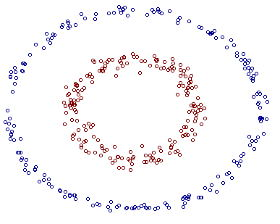
\includegraphics[scale=0.6]{./Pictures/kernel2D.jpg}
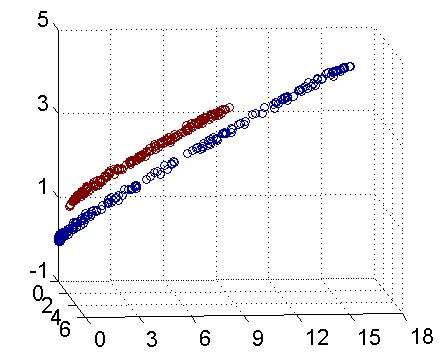
\includegraphics[scale=0.6]{./Pictures/kernel3D.jpg}
\caption{两类数据分别在1)二维空间 ~~~ 2)三维空间}
\label{Fig2D3D}
\end{figure}
从图\ref{Fig2D3D}中可以看出,在二维空间中不可分的两类数据,投影到高维空间利用坐标轴旋转可以实现分类,也就是说利用核函数将数据投影到高维空间后可以找到超平面将原来不可分的数据实现分类,这样就可以实现将非线性问题近似线性化。这就是KPCA 的出发点,该方法也是最常见的一种处理非线性的方法。为了更好地将这种方法应用于过程监测当中来,Lee等人提出了平方预测误差(SPE)的计算方法,由此,$T^2$和SPE 两个统计指标被用到KPCA当中来检测过程。然而,这两个统计指标的置信限计算方法都是假设输入数据服从高斯分布,但是考虑到过程的非线性这种假设在实际的生产过程当中并不能很好地被满足。Ge 等人将统计局部方法引入KPCA 中,利用统计局部方法通过假设检验重新构造了两个检测指标,新的构造的检测指标能够较好的满足高斯分布,从而使得故障的检测率较高地提高。Samuel等则是利用核密度估计(KDE)的方法计算监测指标的控制限,这也在一定程度上改善了监测质量,然而,这也是建立在一定的假设基础上的。但是KPCA应用于过程检测时,依旧需要满足的假设条件是数据服从高斯分布,该假设在实际的生产过程中是不可能满足的,而KECA则是从信息熵的角度出发,不再要求原始数据服从高斯分布,从而与KPCA 相比有更好的检测效果。\\
KECA的原理与KPCA有所不同,在KPCA中考虑到方差对应于数据的特征幅度变化方向,降维则是通过尽可能多的保留数据特征变化来实现,也就是要通过保留核矩阵最大的方差来实现;而KECA则是通过引入信息熵的概念,通过保留最大的信息熵来实现姜维的目的。熵则是通过核矩阵利用Parzen窗实现其密度估计,此时,通过将数据投影到保留输入数据最大熵对应的核方向上实现了维数的降低。然而,在实际的生产过程中会存在不同类型的故障,利用单一的模型并不能够很好地实现对多类型故障的检测。此外,核参数的选择也会对故障的检测效果有重要的影响,恰当的核参数能够使得KECA 对特定的故障有非常好的检测效果。\\
综合以上两方面的考虑,本章提出了利用集成学习通过将多个模型组合起来可以很好的避免由于单个模型选择有误造成的不好的结果,通过选择一系列的多样的能够满足不同故障检测效果核参数建立KECA的子模型,然后将这些子模型通过贝叶斯推论转化为概率的形式,再利用集成学习将这些模型组合起来。此时,检测效果好的模型会有一个较大的权重,这样,模型的监测效果会有较大的改善。这种情况下,不再需要原始数据及降维后的数据服从高斯分布,同时也降低了针对不同类型故障选择合适核参数时候的盲目性。

\section{基于集成学习和贝叶斯网络的模型}
\subsection{KECA模型介绍}
KECA是由特罗姆瑟大学教授Robert Jenssen在2010年提出的,该方法的出发点是信息熵,利用信息熵提取数据中的主成分,将熵最大的方向作为投影方向,从而实现了将高维数据向低维的映射,通过对数据的空间变化达到了特征提取的目的。该方法也被广泛地应用于聚类、模式识别以及降低噪声等领域。
Renyi熵作为一种信息熵的指标,其计算公式为:
\begin{equation}
\label{Equ:entropy}
H(p)=-log\int p^2(X)dX
\end{equation}\\
其中,$p(X)$是样本$X$的概率密度函数,$X$是中心化之后的样本数据。由于对数函数具有单调性,出于简化的目的,式\ref{Equ:entropy}可以考虑为下式:
\begin{equation}
\label{Equ:v_p}
V(p)= \int p^2(X)dX
\end{equation}\\
这样对于瑞利熵$H(p)$的计算转化为对$V(p)$的估计,在此引入Parzen窗概率密度估计算子
\begin{equation}
\label{Equ:parzen}
\^{p}(X)=\frac{1}{N}\sum \limits_{i=1}^{N}k(X,X_t)
\end{equation}\\
其中,$k(X,X_t)$就是parzen窗,也就是中心在$X_t$的核,其性质由参数$c$决定。由于$\^{p}(X)$是密度函数,为了使得其具有较好的性质,那么,$k(X,X_t)$也必须满足是一种密度函数。也就是说此处的parzen窗可以看作是Mercer特征空间中的核函数。通过将公式
(\ref{Equ:parzen})引入到公式(\ref{Equ:v_p})中可以得到:
\begin{equation}\label{estimate}
\hat{V}(p)=\frac{1}{N^2}\sum \limits_{i=1}^{N}\sum \limits_{j=1}^{N}k(X,X_t)=\frac{1}{N^2}\textbf{1}^T\textbf{K}\textbf{1},
\end{equation}
$\textbf{K}$是($N\times N$)的核矩阵,$\textbf{1}$是($N\times 1$)的向量,并且向量中的所有元素都是1。 此时,核矩阵包含了瑞利熵估计中的所有的有效样本。再对核矩阵进行特征分解:
\begin{equation}
\textbf{K}=\textbf{E}\Lambda\textbf{E}^T,
\end{equation}
$\textbf{E}$是分解之后的特征向量矩阵,矩阵中每一列为特征分解的特征向量$\mathbf{e}_1,...,\mathbf{e}_N$,$\Lambda$为其特征矩阵,该矩阵为对角矩阵,对角线上所有元素就是其对应的特征值$\lambda_1,...,\lambda_N$。 此时,公式(\ref{estimate})可以表示为
\begin{equation}\label{eigdec}
\hat{V}(p)=\frac{1}{N^2}\sum \limits_{i=1}^{N}(\sqrt\lambda_i \mathbf{e}_i^T\textbf{1})^2.
\end{equation}%\newline
也就是说,瑞利熵可以表示为$N$个分量的累积,每一个分量都对熵的估计起一定的作用,而这个分量即包含了特征值又包含了特征向量。而当且仅当$\lambda_i \neq 0$或 $\sqrt\lambda_i\mathbf{e}_i^T\textbf{1} \neq 0$时候,该累积项才会对熵估计有贡献。这就是说,单独的特征值无论其值的大小并不能够保证对瑞利熵有一个较大的贡献值。
\subsection{KECA的优势}
KECA与KPCA是两种比较相似的数据转换方法,但是两者却是从不同的角度出发的,KECA具备一定的优势,其具体表现为:\\
(1)信息熵角度出发\\
KECA与KPCA相比一个优势就在于KECA不需要任何的假设前提。KPCA是为了解决PCA针对非线性情况下监测效果恶化的问题,该方法依旧需要原始数据服从高斯分布的假设条件,而KECA则是从信息熵的角度出发,通过实现据集的平均向量欧几里德长度的估计达到数据变换。而在实际的工业过程当中获得的数据并不是满足高斯分布,KECA在原理上相较于KPCA更具有优势。\\
(2)核矩阵中心化\\
在KECA将数据映射到特征空间后,核矩阵并不需要中心化,因为核矩阵的中心化意味着$m=\frac{1}{N}\sum\Phi(X)=0$,而$\hat{V}(p)=\|m\|^2=0$,那么,瑞利熵的估计$\hat{H}(p)=\infty$,输入空间的瑞利熵的估计值为无穷大。由此,针对大规模数据时,该方法在实现过程中可以减少计算量。\\
(3)角结构\\
KECA方法在将数据映射的过程中,投影后的数据会有一个很明显的角结构,这就使得数据经过KECA后能够更好地区分开来,而KPCA并不具备这样的能力。
